\section{Electron self-energy from phonons}\label{sec:6.3}

At \SI{10}{mK} a silicon crystal holds no thermal phonons, yet its band gap is about \SI{60}{meV} smaller than the gap of the same crystal with its nuclei frozen at their equilibrium positions. The zero-point motion of \cref{sec:5.3}, with a root-mean-square amplitude of \SI{0.05}{\angstrom} along each axis, moves the bands by an amount that matters near threshold: the lightest dark-matter mass a detector can see scales with the gap (\cref{eq:1.3-mmin}). The same coupling decides how long a conduction electron with a few meV of excess energy keeps that energy before it hands it to the lattice. Both effects are the electron self-energy of \cref{sec:4.7}, with phonons as the boson.

\subsection{Fan--Migdal and Allen--Heine terms}

A displaced nucleus changes the potential that the electrons feel, at first and at second order in the displacement. Expanding the self-consistent potential $V_{\mathrm{KS}}$ about equilibrium,
\begin{equation*}
  V_{\mathrm{KS}} = V^{(0)}_{\mathrm{KS}} + \sum_a\frac{\partial V_{\mathrm{KS}}}{\partial u_a}\,u_a + \frac12\sum_{ab}\frac{\partial^2V_{\mathrm{KS}}}{\partial u_a\,\partial u_b}\,u_au_b ,
\end{equation*}
with $a = (\vect{R}\kappa\alpha)$ running over cells, species and Cartesian directions. The linear term is the electron--phonon Hamiltonian $H_{\mathrm{ep}}$ of \cref{eq:6.1-Hep}, with the screened vertex $g_{mn\nu}(\vect{k},\vect{Q})$ of \cref{sec:6.2}. The quadratic term, with each displacement expanded in normal modes by \cref{eq:A.6-u}, is a vertex with two phonon operators,
\begin{equation}
  \begin{gathered}
  H^{(2)}_{\mathrm{ep}} = \frac1N\sum_{\vect{k}\vect{Q}\vect{Q}'}\sum_{mn\nu\nu'}g^{\mathrm{AH}}_{mn\nu\nu'}(\vect{k},\vect{Q},\vect{Q}')\,c^\dagger_{m,\vect{k}+\vect{Q}+\vect{Q}'}c_{n\vect{k}}\,B_{\vect{Q}\nu}B_{\vect{Q}'\nu'} , \\
  g^{\mathrm{AH}}_{mn\nu\nu'}(\vect{k},\vect{Q},\vect{Q}') = \frac{1}{2}\sum_{\kappa\alpha,\kappa'\beta}\frac{e^\alpha_{\kappa\nu}(\vect{Q})\,e^\beta_{\kappa'\nu'}(\vect{Q}')}{\sqrt{2M_\kappa\omega_{\vect{Q}\nu}\,2M_{\kappa'}\omega_{\vect{Q}'\nu'}}}\,\bigl\langle\psi_{m,\vect{k}+\vect{Q}+\vect{Q}'}\big|\partial^2_{\kappa\alpha\vect{Q},\kappa'\beta\vect{Q}'}V_{\mathrm{KS}}\big|\psi_{n\vect{k}}\bigr\rangle ,
  \end{gathered}
  \label{eq:6.3-HAH}
\end{equation}
where $\partial^2_{\kappa\alpha\vect{Q},\kappa'\beta\vect{Q}'}V_{\mathrm{KS}}$ is the second derivative with respect to two displacement waves, the sum over $\vect{R}$ and $\vect{R}'$ of $\ee^{\ii\vect{Q}\cdot\vect{R}+\ii\vect{Q}'\cdot\vect{R}'}$ times the second derivative with respect to $u^\alpha_{\vect{R}\kappa}$ and $u^\beta_{\vect{R}'\kappa'}$ (\cref{app:D.16}). This is the Allen--Heine vertex $g^{\mathrm{AH}}$ (\cref{app:A.6}). In the energy of an electron, $H_{\mathrm{ep}}$ enters at second order and $H^{(2)}_{\mathrm{ep}}$ at first order, and both carry two factors of the zero-point length $\ell_{\vect{Q}\nu}$: they are of the same order, $\langle u^2\rangle$, and a consistent theory keeps both. We will see below that dropping either violates translation invariance.

The first term is the boson-exchange diagram of \cref{sec:4.8} (\cref{fig:4-diagrams}c): the electron emits or absorbs a phonon, propagates in another band and wavevector, and reabsorbs or re-emits it. Compared with \cref{eq:4.8-sigmaboson}, the vertex carries $1/\sqrt N$ instead of $1/\sqrt \Vol$ and band indices, and the intermediate electron can be in any band $m$. The second term needs no propagator at all. Its two phonon operators are contracted with each other, a phonon line that leaves and returns to the same point of the electron line, and the pair is replaced by its thermal average $\langle B_{\vect{Q}\nu}B_{-\vect{Q}\nu}\rangle = 2n_{\vect{Q}\nu} + 1$. \Cref{app:D.16} carries out the Matsubara sum and the continuation for both diagrams.
\begin{keyresult}[Fan--Migdal and Allen--Heine self-energies]
For a nondegenerate band $n$ at wavevector $\vect{k}$, with energies $\omega$ and $\xi_{m\vect{p}} = \varepsilon_{m\vect{p}} - \mu_{\mathrm{ch}}$ measured from the chemical potential, $f_{m\vect{p}} = n_{\mathrm{F}}(\xi_{m\vect{p}})$ and $n_{\vect{Q}\nu} = n_{\mathrm{B}}(\omega_{\vect{Q}\nu})$,
\begin{gather}
  \begin{aligned}
  \Sigma^{\mathrm{FM}}_{n\vect{k}}(\omega) = \frac1N\sum_{\vect{Q}\nu m}|g_{mn\nu}(\vect{k},\vect{Q})|^2
  \biggl[&\frac{n_{\vect{Q}\nu} + 1 - f_{m,\vect{k}+\vect{Q}}}{\omega - \xi_{m,\vect{k}+\vect{Q}} - \omega_{\vect{Q}\nu} + \ii0^+} \\
  &+ \frac{n_{\vect{Q}\nu} + f_{m,\vect{k}+\vect{Q}}}{\omega - \xi_{m,\vect{k}+\vect{Q}} + \omega_{\vect{Q}\nu} + \ii0^+}\biggr] ,
  \end{aligned}
  \label{eq:6.3-FM}\\
  \Sigma^{\mathrm{AH}}_{n\vect{k}} = \frac1N\sum_{\vect{Q}\nu}g^{\mathrm{AH}}_{nn\nu\nu}(\vect{k},\vect{Q},-\vect{Q})\,(2n_{\vect{Q}\nu} + 1) .
  \label{eq:6.3-AH}
\end{gather}
The Fan--Migdal term depends on frequency and has an imaginary part; the Allen--Heine term is static and real.
\end{keyresult}
\Cref{eq:6.3-FM} is the second-order self-energy of Fan~\cite{fan1951temperature}, called the Migdal self-energy in the theory of metals~\cite{migdal1958interaction}, and \cref{eq:6.3-AH} is the term added by Allen and Heine~\cite{allen1976theory}; together they are Ref.~\cite[Eqs.~(157), (158), (160) and~(161)]{giustino2017electron}. The thermal factors read as in \cref{sec:4.8}. In the emission term, $n + 1$ is stimulated plus spontaneous emission and $-f$ blocks an occupied intermediate state. In the absorption term, $n$ counts the phonons present, and $f$ adds the process in which an electron already in $(m,\vect{k}+\vect{Q})$ emits a phonon and drops into the state. The sum over $m$ now runs over occupied bands as well. For a degenerate level, such as the threefold valence maximum of silicon (\cref{sec:3.3}), the self-energy is a matrix in the partners, and the terms between partners, whose denominators vanish, are left out as the term $m = n$ at $\vect{Q} = 0$ is~\cite[Sect.~III\,A]{ponce2015temperature}. Summed over the whole zone, the matrix commutes with the symmetry operations that leave $\vect{k}$ unchanged. On a level whose partners form one irreducible representation it is therefore a multiple of the identity, and every partner shifts by the average of the diagonal elements over the level. This is how the shifts of degenerate band edges below are defined. At $T = 0$ the zero-point motion enters $\Sigma^{\mathrm{FM}}$ through the $1$ of $n + 1$ and through $f$, and $\Sigma^{\mathrm{AH}}$ through the $1$ of $2n + 1$. One more diagram of the same order, a phonon line at zero wavevector ending on a closed electron loop, vanishes because the expansion is made about the minimum of the Born--Oppenheimer surface (\cref{app:D.16}).

The pole of the Dyson equation \cref{eq:4.7-dyson} then sits at the renormalized band energy
\begin{equation}
  \varepsilon^{\mathrm{ren}}_{n\vect{k}} = \varepsilon_{n\vect{k}} + \Real\Sigma^{\mathrm{FM}}_{n\vect{k}}(\varepsilon^{\mathrm{ren}}_{n\vect{k}}) + \Sigma^{\mathrm{AH}}_{n\vect{k}} ,
  \label{eq:6.3-ren}
\end{equation}
with $\omega$ now measured from the same origin as $\varepsilon$, the quasiparticle condition of \cref{eq:4.7-qp}. Its value at $T = 0$, less $\varepsilon_{n\vect{k}}$, is the \emph{zero-point renormalization} (ZPR) of the state, and the ZPR of a gap is that of the conduction state minus that of the valence state. The theory built on the two terms, usually in the adiabatic form below and with the rigid-ion approximation of Allen and Cardona~\cite{allen1981temperature}, is called Allen--Heine--Cardona (AHC) theory. In practice $\Sigma^{\mathrm{FM}}$ is often evaluated at $\omega = \varepsilon_{n\vect{k}}$ rather than at the solution of \cref{eq:6.3-ren}; for the Einstein boson of \cref{we:4-einstein} the two choices yield \SI{-9.14}{meV} and \SI{-8.73}{meV}, a difference set by $1 - z_{\mathrm{qp}}$.

\subsection{The adiabatic limit}

Where the phonon energies are small next to the electronic energy differences that dominate the sum over $m$, they can be dropped from the denominators of \cref{eq:6.3-FM}. Setting also $\omega = \varepsilon_{n\vect{k}}$, the two terms acquire the same denominator, and their numerators add to $(n + 1 - f) + (n + f) = 2n + 1$: the occupations of the intermediate states drop out. The result is the formula of Allen and Heine~\cite{allen1976theory},
\begin{equation}
  \varepsilon^{\mathrm{ren}}_{n\vect{k}} - \varepsilon_{n\vect{k}} = \frac1N\sum_{\vect{Q}\nu}(2n_{\vect{Q}\nu} + 1)\Biggl[\sum_m\frac{|g_{mn\nu}(\vect{k},\vect{Q})|^2}{\varepsilon_{n\vect{k}} - \varepsilon_{m,\vect{k}+\vect{Q}}} + g^{\mathrm{AH}}_{nn\nu\nu}(\vect{k},\vect{Q},-\vect{Q})\Biggr] ,
  \label{eq:6.3-adiabatic}
\end{equation}
Ref.~\cite[Eq.~(167)]{giustino2017electron}. Every mode now enters with the weight $2n_{\vect{Q}\nu} + 1$ of its mean-square displacement (\cref{eq:5.3-B}). Allen and Heine derived \cref{eq:6.3-adiabatic} without diagrams. With the nuclei frozen at displacements $u_a$, a band energy is a function $\varepsilon_{n\vect{k}}(\{u\})$, and second-order perturbation theory gives its curvature: the Fan sum is the second-order term of $H_{\mathrm{ep}}$, the Allen--Heine vertex the first-order term of the quadratic potential (\cref{eq:D.16-frozen}). The nuclei are not frozen, however, but spread over a Gaussian distribution of width $\langle u_au_b\rangle$. Averaged over it, the linear term vanishes and the energy shifts by half the curvature times the width, $\tfrac12\sum_{ab}\langle u_au_b\rangle\,\partial^2\varepsilon_{n\vect{k}}/\partial u_a\partial u_b$. In the adiabatic limit the AHC shift is the average of the band energy over the zero-point and thermal smearing of the lattice.

The adiabatic form fails where the dropped phonon energies are not small. That happens for $m = n$ at small $Q$, where $\varepsilon_{n\vect{k}} - \varepsilon_{n,\vect{k}+\vect{Q}}$ vanishes with $Q$, and wherever another band is degenerate with the state. Both occur at band edges, the states that set a detector's threshold. The Fr\"ohlich vertex of a polar crystal shows how badly it can fail. Take an electron at the bottom of a parabolic band of mass $m^*$ at $T = 0$, coupled to the longitudinal optical phonon by $|g^{\mathrm{L}}|^2 = C_{\mathrm{F}}^2/Q^2$ (\cref{eq:6.2-frohlich}). In the adiabatic form its intraband Fan term is
\begin{equation*}
  \frac1N\sum_{\vect{Q}}\frac{|g^{\mathrm{L}}|^2}{-Q^2/2m^*} = -\Omega\int\frac{\dd^3Q}{(2\pi)^3}\,\frac{2m^*C_{\mathrm{F}}^2}{Q^4} = -\frac{\Omega\,m^*C_{\mathrm{F}}^2}{\pi^2}\int_0\frac{\dd Q}{Q^2} ,
\end{equation*}
which diverges at small $Q$. The divergence is an artifact. With the phonon energy kept, only the emission term of \cref{eq:6.3-FM} survives for an empty band at $T = 0$, its denominator at $\omega = \varepsilon_{n\vect{k}}$ is $-Q^2/2m^* - \omega_{\mathrm{L}}$, and $\Real\Sigma^{\mathrm{FM}}$ is the finite second-order shift of \cref{sec:6.2}, $-\alpha_{\mathrm{F}}\omega_{\mathrm{L}} = -\SI{2.6}{meV}$ for the conduction band of GaAs (\cref{we:6-frohlich}). The Fr\"ohlich polaron shift is the Fan--Migdal self-energy at the band bottom. Every infrared-active crystal has this $1/Q^2$ coupling. For all of them the adiabatic ZPR is infinite, and the nonadiabatic form, with the phonon energies in the denominators, is needed to get a number~\cite{ponce2015temperature}. In silicon the vertex has no $1/Q$ term (\cref{sec:6.2}), both forms converge, and they differ by \SI{8}{meV}: \SI{-64.3}{meV} adiabatic and \SI{-56.2}{meV} nonadiabatic for the indirect gap in the local-density approximation~\cite[Table~VI]{ponce2015temperature}.

\subsection{Translation invariance and the rigid-ion approximation}

Moving the whole crystal by a constant vector shifts no band energy. For long-wavelength acoustic phonons this ties the Fan and Allen--Heine terms together. As $Q \to 0$ an acoustic mode becomes a rigid translation, with $\vect{e}_{\kappa\nu} \to (M_\kappa/M_{\mathrm{cell}})^{1/2}\hat{\vect{e}}_\nu$ and every nucleus displaced by $\ell_{\vect{Q}\nu}\hat{\vect{e}}_\nu/\sqrt N$ per unit of $B_{\vect{Q}\nu}$ (\cref{app:A.6}). Its vertex then follows from \cref{eq:6.2-g} and the acoustic sum rule \cref{eq:6.2-asr},
\begin{equation*}
  g_{mn\nu}(\vect{k},\vect{Q}) \to \ell_{\vect{Q}\nu}\sum_\kappa\hat{\vect{e}}_\nu\cdot\bigl\langle\psi_{m\vect{k}}\bigr|\partial_{\kappa,\vect{0}}V_{\mathrm{KS}}\bigl|\psi_{n\vect{k}}\bigr\rangle = -\ii\,\ell_{\vect{Q}\nu}\,(\varepsilon_{n\vect{k}} - \varepsilon_{m\vect{k}})\,\hat{\vect{e}}_\nu\cdot\vect{p}_{mn}(\vect{k}) .
\end{equation*}
The intraband element vanishes, as \cref{sec:6.2} showed; the interband elements do not. In the Fan sum of \cref{eq:6.3-adiabatic} the energy difference is squared in the numerator and appears once in the denominator. What is left is
\begin{equation*}
  \sum_{m\ne n}\frac{|g_{mn\nu}|^2}{\varepsilon_{n\vect{k}} - \varepsilon_{m\vect{k}}} \to \ell_{\vect{Q}\nu}^2\sum_m(\varepsilon_{n\vect{k}} - \varepsilon_{m\vect{k}})\,|\hat{\vect{e}}_\nu\cdot\vect{p}_{mn}|^2 .
\end{equation*}
For the Allen--Heine vertex of the same mode, the same polarization vectors turn the prefactor of \cref{eq:6.3-HAH} into $\ell_{\vect{Q}\nu}^2\hat e_{\nu\alpha}\hat e_{\nu\beta}$, and the second derivative with respect to two displacement waves of zero wavevector, summed over $\kappa$ and $\kappa'$, becomes the second derivative with respect to a uniform translation $\vect{t}$ of the whole crystal. The self-consistent potential moves with the crystal, $V_{\mathrm{KS}} \to \op{T}_{\vect{t}}V_{\mathrm{KS}}\op{T}^\dagger_{\vect{t}}$ with $\op{T}_{\vect{t}} = \ee^{-\ii\vect{t}\cdot\op{\vect{p}}}$ (\cref{sec:6.2}). Differentiating twice along $\hat{\vect{e}}_\nu$ gives $-[\op{p}_\nu,[\op{p}_\nu,V_{\mathrm{KS}}]]$ with $\op{p}_\nu = \hat{\vect{e}}_\nu\cdot\op{\vect{p}}$, and since the kinetic energy commutes with $\op{p}_\nu$, $V_{\mathrm{KS}}$ may be replaced by $H_{\mathrm{KS}}$. Expanding the double commutator in the eigenstates of $H_{\mathrm{KS}}$ at $\vect{k}$, the states that $\op{p}_\nu$ connects to $\psi_{n\vect{k}}$,
\begin{equation*}
  g^{\mathrm{AH}}_{nn\nu\nu}(\vect{k},\vect{Q},-\vect{Q}) \to -\frac{\ell_{\vect{Q}\nu}^2}{2}\bigl\langle\psi_{n\vect{k}}\bigr|[\op{p}_\nu,[\op{p}_\nu,H_{\mathrm{KS}}]]\bigl|\psi_{n\vect{k}}\bigr\rangle = -\ell_{\vect{Q}\nu}^2\sum_m(\varepsilon_{n\vect{k}} - \varepsilon_{m\vect{k}})\,|\hat{\vect{e}}_\nu\cdot\vect{p}_{mn}|^2 .
\end{equation*}
The two contributions cancel term by term:
\begin{equation}
  \sum_{m\ne n}\frac{|g_{mn\nu}(\vect{k},\vect{Q})|^2}{\varepsilon_{n\vect{k}} - \varepsilon_{m,\vect{k}+\vect{Q}}} + g^{\mathrm{AH}}_{nn\nu\nu}(\vect{k},\vect{Q},-\vect{Q}) \to 0 \qquad (\nu \text{ acoustic},\ Q \to 0) .
  \label{eq:6.3-cancel}
\end{equation}
The picture is the one of \cref{sec:6.2}. The interband vertex translates the electronic state along with the crystal, and at second order it shifts the energy by $\ell_{\vect{Q}\nu}^2\sum_m(\varepsilon_{n\vect{k}} - \varepsilon_{m\vect{k}})|\hat{\vect{e}}_\nu\cdot\vect{p}_{mn}|^2$, a sum of either sign: bands above $n$ push it down, bands below push it up. The Allen--Heine term measures the curvature of the potential under the same translation, and it shifts the energy back by exactly as much. Neither term means anything alone, and a calculation must treat both on the same grid of wavevectors. In the language of scalar quantum electrodynamics (QED) the two are the rainbow and the seagull diagrams, and their cancellation for a rigid translation is the analogue of the one that makes the scattering of low-frequency light by a bound electron vanish. The same double commutator underlies the f-sum rule (\cref{eq:4.3-firstmoment}). The three translational modes at exactly $\vect{Q} = 0$, with zero frequency, are left out of both sums; \cref{eq:6.3-cancel} states that the integrand is continuous there. For small $Q$ the first correction to the cancellation is linear in $\vect{Q}$ and drops out of the sum over directions. The interband remainder is then smaller by a factor $\sim Q^2$, and long-wavelength acoustic phonons, which carry a large share of the thermal $\langle u^2\rangle$ of silicon (\cref{we:5-u2}), barely shift the bands. What survives at small $Q$ is the intraband term, $m = n$, whose denominator vanishes with $Q$, the term that needs the phonon energy kept.

The Allen--Heine vertex needs second derivatives of the self-consistent potential, a second-order perturbation calculation that few codes perform. Translation invariance offers a way around it. A rigid translation leaves every band energy unchanged at every configuration of the nuclei, so the sum over all nuclei of $\partial\varepsilon_{n\vect{k}}/\partial u_{\vect{R}\kappa\alpha}$ vanishes everywhere, and so does its derivative. At equilibrium this is an exact sum rule, \cref{eq:D.16-sr2}: the diagonal element of the second derivative, summed over the sites of the whole crystal, equals a product of first derivatives at $\vect{Q} = 0$. The sum rule fixes a sum over sites, while $g^{\mathrm{AH}}$ needs the on-site element. The \emph{rigid-ion approximation} supplies the missing step. It writes the potential as a sum of atom-centered terms that move rigidly with their nuclei, $V_{\mathrm{KS}} = \sum_{\vect{R}\kappa}v_\kappa(\vect{r} - \vect{R} - \vect{\tau}_\kappa - \vect{u}_{\vect{R}\kappa})$. Second derivatives with respect to two different atoms then vanish, the sum rule determines the on-site element (\cref{eq:D.16-ria}), and the Allen--Heine term becomes
\begin{equation}
  \Sigma^{\mathrm{AH}}_{n\vect{k}} = -\frac12\sum_{\kappa\kappa'}\sum_{\alpha\beta}\bigl(B^{\alpha\beta}_\kappa + B^{\alpha\beta}_{\kappa'}\bigr)\,\Real{\sum_{m}}'\frac{\langle\psi_{n\vect{k}}|\partial_{\kappa\alpha,\vect{0}}V_{\mathrm{KS}}|\psi_{m\vect{k}}\rangle\,\langle\psi_{m\vect{k}}|\partial_{\kappa'\beta,\vect{0}}V_{\mathrm{KS}}|\psi_{n\vect{k}}\rangle}{\varepsilon_{n\vect{k}} - \varepsilon_{m\vect{k}}} ,
  \label{eq:6.3-ria}
\end{equation}
where $B_\kappa = \langle\vect{u}_\kappa\vect{u}_\kappa\rangle$ is the displacement tensor of \cref{eq:5.3-B} at temperature $T$ and the prime excludes the states degenerate with $(n,\vect{k})$ (\cref{app:D.16}). This is the form of Allen and Cardona~\cite{allen1981temperature}, Ref.~\cite[Eqs.~(195)--(198)]{giustino2017electron}. It needs just the first-order potentials at $\vect{Q} = 0$, which every phonon calculation already supplies. Its structure is a Fan term at zero wavevector with the opposite sign, weighted by the mean-square displacement of each atom; the cancellation of \cref{eq:6.3-cancel} is built in. What it neglects is the change of screening when two atoms move together rather than one at a time. Poncé et al.\ find that correction large in molecules~\cite{ponce2015temperature}; for crystals the rigid-ion form is the standard choice.

In practice the AHC shift is computed from DFPT vertices on a grid of phonon wavevectors. The sum over bands is split into an active window, summed explicitly, and the rest, obtained from a Sternheimer equation. The sum over $\vect{Q}$ converges slowly near the vanishing intraband denominators and needs grids of $10^5$ to $10^6$ points, or Wannier interpolation of the vertex (\cref{sec:6.2}), with a small imaginary part in the denominators extrapolated to zero. \Cref{app:E.8} describes the calculation, its convergence parameters and its pitfalls, among them the small residual Born charges of a nonpolar DFPT calculation, which must be removed before the sum or the integral diverges at a band extremum.

\subsection{Smeared ionic potentials}

The literature calls $\Sigma^{\mathrm{AH}}$ the Debye--Waller self-energy, and in the rigid-ion approximation the name has a reason. Average the rigid-ion potential over the Gaussian distribution of the displacements of each nucleus. A Fourier component $v_\kappa(\vect{G})\,\ee^{\ii\vect{G}\cdot(\vect{r} - \vect{R} - \vect{\tau}_\kappa)}$ acquires the factor $\langle\ee^{-\ii\vect{G}\cdot\vect{u}_\kappa}\rangle = \ee^{-\vect{G}\cdot B_\kappa\cdot\vect{G}/2}$, and to first order in $B_\kappa$
\begin{equation}
  \bigl\langle v_\kappa(\vect{r} - \vect{u}_\kappa)\bigr\rangle - v_\kappa(\vect{r}) = \frac12\sum_{\alpha\beta}B^{\alpha\beta}_\kappa\,\partial_\alpha\partial_\beta v_\kappa(\vect{r}) = -\sum_{\vect{G}}W_\kappa(\vect{G})\,v_\kappa(\vect{G})\,\ee^{\ii\vect{G}\cdot\vect{r}} ,
  \label{eq:6.3-smear}
\end{equation}
for the atom at the origin, with $2W_\kappa(\vect{G}) = \vect{G}\cdot B_\kappa\cdot\vect{G}$, the exponent of \cref{eq:5.6-W} evaluated at a reciprocal-lattice vector. The diagonal matrix element of the middle expression, summed over all the sites of every species, is the rigid-ion Allen--Heine term (\cref{app:D.16}). So $\Sigma^{\mathrm{AH}}$ is the first-order change of a band energy when each ionic potential is smeared out by the zero-point and thermal motion of its nucleus, the ``fuzziness'' of the nuclear charge described in Ref.~\cite[below Eq.~(154)]{giustino2017electron}.

It is nonetheless a different object from the Debye--Waller factor $\ee^{-2W_\kappa(\vect{q})}$ of \cref{sec:5.6}, a probability that multiplies a rate at the momentum transfer of the scattering. The smearing of \cref{eq:6.3-smear} involves no momentum transfer and no rate. It is evaluated at the reciprocal-lattice vectors of the static potential, enters an energy at first order in $B_\kappa$, and is one of the two terms of the second-order shift. The Fan term is of the same order and partly cancels it, exactly so for acoustic phonons at small $Q$ (\cref{eq:6.3-cancel}). Allen and Heine showed that a theory of the band shifts with the smeared potential alone is incomplete~\cite{allen1976theory}. The two share the displacement tensor $B_\kappa$, and nothing else.

\subsection{Zero-point renormalization}

For the indirect gap of silicon, AHC theory in the local-density approximation gives a zero-point renormalization of \SI{-56.2}{meV} in the nonadiabatic form~\cite[Table~VI]{ponce2015temperature}. The valence maximum rises and the conduction minimum drops, by \SI{35}{meV} and \SI{22}{meV} in a calculation by a different method~\cite[Sect.~VII\,B]{zacharias2020theory}, and the gap closes from both sides. That calculation used \emph{special displacements}, a non-perturbative route that avoids vertices and sums over wavevectors altogether. Since the adiabatic shift is the average of the band energy over the Gaussian distribution of the nuclei, it can be computed directly: displace the nuclei of a large supercell and compute the bands. Zacharias and Giustino showed that a single configuration suffices, one in which every normal coordinate has its root-mean-square amplitude and the signs alternate between modes so that the cross terms cancel~\cite{zacharias2016one}. In an $8\times8\times8$ supercell of 1024 atoms it yields \SI{-57}{meV}~\cite[Sect.~VII\,B]{zacharias2020theory}. The method includes all orders in the displacements but is adiabatic by construction.

The renormalization extracted from experiment is \SI{-62}{meV} or \SI{-64}{meV}, depending on the route~\cite{cardona2005electron}, as tabulated in Ref.~\cite[Table~VI]{ponce2015temperature}. A ZPR cannot be measured directly, since no experiment freezes the nuclei. Both routes rest on how the shift depends on temperature and on the nuclear mass, which the simplest model makes explicit.

Suppose every phonon has the same energy $\omega_{\mathrm{Ein}}$, an Einstein crystal. The weight $2n_{\vect{Q}\nu} + 1 = \coth(\omega_{\mathrm{Ein}}/2T)$ is then the same for every mode and comes out of the sum in \cref{eq:6.3-adiabatic}. The shift of any band at temperature $T$ is its zero-point value times one function of temperature,
\begin{equation}
  \Delta\varepsilon_{n\vect{k}}(T) = \Delta\varepsilon_{n\vect{k}}(0)\,\coth\frac{\omega_{\mathrm{Ein}}}{2T} .
  \label{eq:6.3-einstein}
\end{equation}
At $T \gg \omega_{\mathrm{Ein}}$, $\coth x \simeq 1/x + x/3$, and the shift becomes linear in $T$ with the slope $2\Delta\varepsilon(0)/\omega_{\mathrm{Ein}}$. Since this line extrapolates to zero shift at $T = 0$, extrapolating a measured gap back from high temperature lands on the gap of the clamped lattice, and the low-temperature gap sits below that intercept by the ZPR. This is one of the two extractions. The other uses the nuclear mass. At fixed force constants $\omega_{\mathrm{Ein}} \propto M^{-1/2}$, the squared vertex and the Allen--Heine term are both proportional to $\ell^2 \propto 1/(M\omega_{\mathrm{Ein}}) \propto M^{-1/2}$, and so is the ZPR. Then $\mathrm{ZPR} = -2M\,\partial\Eg/\partial M$, and the gaps of isotopically enriched crystals measure it.

\begin{workedexample}{The Einstein model of the silicon gap}\label{we:6-zpr}
The Einstein boson of \cref{we:4-einstein} shifted the band bottom by \SI{-9.14}{meV} at $T = 0$ and by \SI{-11.09}{meV} at \SI{300}{K}, a ratio of 1.213 against $2n_{\mathrm{B}} + 1 = 1.218$. The small difference came from the boson energy in the denominators. In the adiabatic limit \cref{eq:6.3-einstein} makes the ratio exact, and the model reduces to two numbers: the ZPR and $\omega_{\mathrm{Ein}}$.

For silicon we choose $\omega_{\mathrm{Ein}}$ by the zero-point motion. At $T = 0$ every term of the ZPR carries a factor $1/\omega_{\vect{Q}\nu}$ from $\ell_{\vect{Q}\nu}^2$, as the mean-square displacement does, and the Einstein energy that reproduces the zero-point $\langle u^2\rangle$ of the computed phonon spectrum is $\langle\omega^{-1}\rangle^{-1} = \SI{30.4}{meV}$, or \SI{353}{K} (\cref{we:5-u2}). For the ZPR we take the nonadiabatic AHC value, \SI{-56.2}{meV}. Applying the adiabatic weight of \cref{eq:6.3-einstein} to a nonadiabatic value is an approximation; the two forms differ by \SI{8}{meV} at $T = 0$.

At \SI{300}{K}, $T = \SI{25.85}{meV}$, $\omega_{\mathrm{Ein}}/2T = 0.588$ and $\coth(0.588) = 1.891$. The model predicts that the gap closes between zero and room temperature by
\begin{equation*}
  \Eg(\SI{300}{K}) - \Eg(0) = -\SI{56.2}{meV}\times(1.891 - 1) = -\SI{50.1}{meV} .
\end{equation*}
The measured gap, $\Eg(T) = \Eg(0) - aT^2/(T + b)$ with $\Eg(0) = \SI{1.1692}{eV}$, $a = \SI{4.9e-4}{eV.K^{-1}}$ and $b = \SI{655}{K}$, a fit to photoluminescence up to \SI{1000}{K}~\cites{alex1996temperature}[Eq.~(11)]{ramanathan2020ionization}, falls by \SI{46.2}{meV}, from \SI{1.1692}{eV} to \SI{1.1230}{eV}. The model is \SI{8}{\percent} high; with the adiabatic ZPR, \SI{-64.3}{meV}, it would predict \SI{-57.3}{meV}. Its high-temperature slope is $2\times\SI{56.2}{meV}/\SI{353}{K} = \SI{0.318}{meV.K^{-1}}$, between the slopes of the measured curve at \SI{300}{K} and \SI{500}{K}, 0.26 and \SI{0.33}{meV.K^{-1}}.

The choice of $\omega_{\mathrm{Ein}}$ carries physics. Had we assumed that the gap follows the full mean-square displacement of the computed spectrum, the shift would have scaled with $\langle u^2\rangle(T)/\langle u^2\rangle(0) = 2.661$, and the gap would have closed by $\SI{56.2}{meV}\times1.661 = \SI{93.3}{meV}$ at \SI{300}{K}, twice the measured value. That assumption gives every mode a shift in proportion to its mean-square displacement, and the thermal $\langle u^2\rangle$ is weighted toward the softest modes, which enter with $1/\omega^2$: the long-wavelength acoustic phonons and the flat transverse acoustic branches near the zone boundary (\cref{we:5-u2}). The measured curve says that these modes move the gap less than their share of $\langle u^2\rangle$, and for the acoustic modes at small $Q$ \cref{eq:6.3-cancel} explains why: they are nearly rigid translations. The gap responds to the displacements of atoms relative to their neighbors, not to their displacement as such.

Two further numbers follow. The model's clamped-lattice gap, the intercept of its high-temperature line, is $\SI{1.1692}{eV} + \SI{0.0562}{eV} = \SI{1.2254}{eV}$; the model is anchored at the measured $\Eg(0)$, which contains the zero-point expansion of the lattice, and it leaves out thermal expansion. And replacing natural silicon, $M = \SI{28.09}{u}$, by $^{30}$Si scales the ZPR by $(28.09/29.97)^{1/2}$ and raises the gap by \SI{1.8}{meV}. At detector temperatures nothing of the thermal part survives. At \SI{1}{K}, $\omega_{\mathrm{Ein}}/T = 353$ and $2n_{\mathrm{B}}(\omega_{\mathrm{Ein}}) \sim 10^{-153}$; the only phonons still occupied are acoustic modes at small $Q$, and their contribution vanishes by \cref{eq:6.3-cancel} and with their phase space. A detector at \SI{10}{mK} therefore sees $\Eg(0)$.
\end{workedexample}

\begin{figure}[tbp]
  \centering
  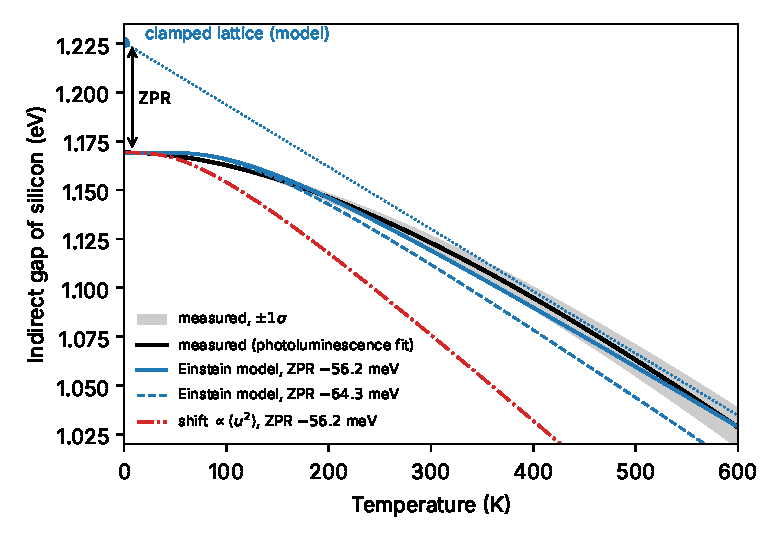
\includegraphics[width=0.8\linewidth]{figures/ch06/fig6_4.pdf}
  \caption{The indirect gap of silicon against temperature. Black: measured, the fit $\Eg(T) = \SI{1.1692}{eV} - aT^2/(T + b)$ with $a = \SI{4.9e-4}{eV.K^{-1}}$ and $b = \SI{655}{K}$ to photoluminescence data~\cite{alex1996temperature,ramanathan2020ionization}; the gray band is the envelope of the fits with $a$ and $b$ varied independently by their quoted errors of \SI{0.2e-4}{eV.K^{-1}} and \SI{40}{K}. Blue: Einstein model $\Eg(0) + \mathrm{ZPR}\,[\coth(\omega_{\mathrm{Ein}}/2T) - 1]$ with $\omega_{\mathrm{Ein}} = \SI{30.4}{meV}$, the Einstein energy that reproduces the zero-point mean-square displacement of the computed phonon spectrum, and the computed zero-point renormalization, \SI{-56.2}{meV} (solid, nonadiabatic) or \SI{-64.3}{meV} (dashed, adiabatic)~\cite{ponce2015temperature}. Red, dash-dotted: a shift proportional to the full mean-square displacement $\langle u^2\rangle(T)$ of the computed spectrum, with the same zero-point value. Blue dotted line and dot: the high-temperature asymptote of the solid model, which extrapolates to the model's clamped-lattice gap, \SI{1.2254}{eV}, at $T = 0$; the arrow marks the ZPR. All model curves are anchored at the measured gap at $T = 0$ and leave out thermal expansion.}
  \label{fig:6-gapT}
\end{figure}

In \cref{fig:6-gapT} the Einstein model with a computed ZPR and an Einstein energy fixed by the zero-point motion follows the measured gap to within about \SI{5}{meV} from zero to \SI{600}{K}. Below \SI{150}{K} it falls slightly too slowly, since a single energy of \SI{30}{meV} cannot represent the softer modes that the real spectrum starts to populate first. The curve that follows $\langle u^2\rangle$ fails from the start.

The values \SI{-62}{meV} and \SI{-64}{meV} extracted from experiment come from the isotope dependence of the gap and from the linear extrapolation of its high-temperature part~\cite{cardona2005electron}, and they need no Einstein energy. They contain the whole zero-point shift of the gap, including a part that is not electron--phonon coupling at all: the zero-point motion also expands the lattice, which by itself opens the gap by \SI{9}{meV}~\cite[Table~S2]{miglio2020predominance}. The electron--phonon part implied by experiment is therefore $-71$ to \SI{-73}{meV}. That is the number to compare with the computed \SI{-56.2}{meV}, a fixed-volume electron--phonon value, and the calculation falls about \SI{20}{\percent} short of it, as does the special-displacement value of \SI{-57}{meV}. The shortfall is consistent with the overscreening of the vertex by the small Kohn--Sham gap: a calculation of the same kind on $GW$ bands gives \SI{66}{meV}~\cite[Sect.~VII\,B]{zacharias2020theory}.

\subsection{Phonon-limited lifetimes}

The imaginary part of the self-energy is a decay rate. The Allen--Heine term is real and contributes nothing to it. For the Fan--Migdal term, the Sokhotski--Plemelj formula \cref{eq:2.4-SP} turns each denominator of \cref{eq:6.3-FM} into a delta function,
\begin{equation}
  \begin{aligned}
  \Imag\Sigma^{\mathrm{FM}}_{n\vect{k}}(\omega) = -\frac{\pi}{N}\sum_{\vect{Q}\nu m}|g_{mn\nu}(\vect{k},\vect{Q})|^2
  \Bigl[&(n_{\vect{Q}\nu} + 1 - f_{m,\vect{k}+\vect{Q}})\,\delta(\omega - \xi_{m,\vect{k}+\vect{Q}} - \omega_{\vect{Q}\nu}) \\
  &+ (n_{\vect{Q}\nu} + f_{m,\vect{k}+\vect{Q}})\,\delta(\omega - \xi_{m,\vect{k}+\vect{Q}} + \omega_{\vect{Q}\nu})\Bigr] ,
  \end{aligned}
  \label{eq:6.3-ImFM}
\end{equation}
and by \cref{eq:4.7-qp} the state decays at the rate $\varGamma_{n\vect{k}} = -2z_{\mathrm{qp}}\Imag\Sigma^{\mathrm{FM}}_{n\vect{k}}(\xi_{n\vect{k}})$, its \emph{phonon-limited lifetime} being $1/\varGamma_{n\vect{k}}$. The cutting rule of \cref{sec:4.8} reads \cref{eq:6.3-ImFM} as golden-rule rates: the cut runs through the intermediate electron and the phonon, and puts both on shell. For an electron in an empty band the out-scattering rates are all that remain, emission of a phonon with the weight $n + 1$ and absorption with the weight $n$ of \cref{eq:A.6-weights}.

At $T = 0$ only emission is left, and an electron can emit only if a state of lower energy is available. An electron at the bottom of the conduction band of an insulator has none, and its width is zero: band edges are sharp at zero temperature, as \cref{sec:4.7} anticipated. A width found at a band extremum at $T = 0$ in a calculation is the imaginary part added to the denominators for numerical reasons, not a lifetime. At \SI{10}{mK} the absorption term is absent for every phonon above about \SI{10}{\micro eV}, and a hot carrier in a detector loses its energy by spontaneous emission only. How fast, and down to what energy?

For a conduction electron near a band minimum the answer is set by acoustic phonons. Take a parabolic band of mass $m^*$, an electron of wavevector $\vect{k}$ measured from the minimum, and the deformation-potential vertex $|g|^2 = \Xi^2Q/(2M_{\mathrm{cell}}c)$ of \cref{eq:6.2-D}, for a branch of sound speed $c$ and an effective constant $\Xi$. At $T = 0$, with $(1/N)\sum_{\vect{Q}} \to \Omega\int\dd^3Q/(2\pi)^3$,
\begin{equation*}
  \varGamma(\vect{k}) = 2\pi\,\Omega\int\frac{\dd^3Q}{(2\pi)^3}\,\frac{\Xi^2Q}{2M_{\mathrm{cell}}c}\;\delta\Bigl(\frac{k^2 - |\vect{k} + \vect{Q}|^2}{2m^*} - cQ\Bigr) .
\end{equation*}
The delta function fixes the angle $\theta$ between $\vect{Q}$ and $\vect{k}$ at $\cos\theta = -(Q/2 + m^*c)/k$, and the integral over $\cos\theta$ gives $m^*/(kQ)$. A solution exists only for $Q \le Q_{\max} = 2(k - m^*c)$, which requires $k > m^*c$: the electron must move faster than sound. The emission is Cherenkov radiation of sound, and the phonons go out on a cone about the direction of motion. The remaining integral over $Q$ gives
\begin{equation}
  \varGamma(\vect{k}) = \frac{\Omega\,\Xi^2\,m^*\,Q_{\max}^3}{12\pi M_{\mathrm{cell}}\,c\,k} , \qquad Q_{\max} = 2(k - m^*c) ,
  \label{eq:6.3-cherenkov}
\end{equation}
which grows linearly with the kinetic energy $k^2/2m^*$ far above the threshold.

For silicon we estimate the rate with three simplifications. The valley is taken spherical, with the density-of-states mass $m^* = m^*_{\mathrm{d}} = (m^*_\parallel m^{*2}_\perp)^{1/3} = 0.322\,m_e$ from the valley masses of \cref{sec:3.3}. The valley constants of \cref{sec:6.2}, $\Xi_d = \SI{1.01}{eV}$ and $\Xi_u = \SI{8.84}{eV}$, enter with their angular factors averaged over the angle between $\vect{Q}$ and the valley axis, as for valleys of random orientation: $\Xi^2 = \Xi_d^2 + \tfrac23\Xi_d\Xi_u + \tfrac15\Xi_u^2 = (\SI{4.75}{eV})^2$ for the longitudinal branch and $\tfrac{2}{15}\Xi_u^2 = (\SI{3.23}{eV})^2$ for the one transverse branch that couples. And the sound speeds are the measured ones along $[100]$, 8.43 and \SI{5.84}{km.s^{-1}} (\cref{sec:5.2}). The thresholds $m^*c^2/2$ are \SI{0.065}{meV} for longitudinal and \SI{0.031}{meV} for transverse emission. At \SI{10}{meV} of kinetic energy the two branches give $\varGamma = 7.2 + \SI{5.2}{\micro eV} = \SI{12.3}{\micro eV}$, a lifetime of \SI{53}{ps}; at \SI{1}{meV} the lifetime is \SI{0.9}{ns}, and at \SI{30}{meV} \SI{16}{ps}. Above the optical phonon energy, \SI{64}{meV}, and through intervalley scattering (\cref{sec:6.2}) the rates are far higher. The estimate fixes the scale. An electron created with a few meV in a silicon detector sheds it as acoustic phonons over a fraction of a nanosecond, and then stops emitting once its kinetic energy falls below a few tens of \si{\micro eV}, under \SI{1}{K}. In a biased detector the field keeps the carriers above that threshold, and the phonons emitted along the drift are the Luke phonons of \cref{sec:20.1}. A quantitative rate uses \cref{eq:6.3-ImFM} with DFPT vertices on fine grids and the real anisotropic valleys.

\subsection{Migdal's adiabatic theorem}

The Fan--Migdal self-energy keeps the vertex $g$ bare at both ends and the propagators free. The exact self-energy has the same structure with every piece dressed: the full electron propagator, the full phonon propagator, and a vertex function in place of one of the two $g$'s~\cite[Eq.~(156)]{giustino2017electron}. At fourth order in $g$ two new diagrams appear. In one, a second phonon line is emitted and reabsorbed inside the first, on the intermediate electron line; it is a self-energy insertion, and replacing the free propagator in \cref{eq:6.3-FM} by the full one sums all such insertions. In the other, the two phonon lines cross. This is a vertex correction, and no self-consistency of the propagators includes it. Migdal's question was how large it is~\cite{migdal1958interaction}.

In a metal, the counting of \cref{sec:6.1} answers it. Consider an electron at the Fermi surface. In the self-energy insertion the inner phonon carries a frequency of at most $\omega_{\mathrm{D}}$. The intermediate electron can sit anywhere on the Fermi surface, within $\omega_{\mathrm{D}}$ of it in energy. The insertion is then as large as the self-energy itself, a fraction $\lambda_{\mathrm{ep}}$ of $\omega_{\mathrm{D}}$, with $\lambda_{\mathrm{ep}}$ the dimensionless electron--phonon coupling, defined so that the mass of an electron at the Fermi surface is enhanced by $1 + \lambda_{\mathrm{ep}}$ (\cref{sec:6.4}). In the crossed diagram, two intermediate electron lines carry momenta that differ by the momentum of the outer phonon. Both lie within $\omega_{\mathrm{D}}$ of the Fermi surface only where two thin shells, of thickness $\omega_{\mathrm{D}}/v_{\mathrm{F}}$ with $v_{\mathrm{F}}$ the Fermi velocity and shifted by that momentum, intersect, a fraction $\sim\omega_{\mathrm{D}}/E_{\mathrm{F}}$ of the momenta summed over. Elsewhere one of the two lines is off shell by an energy of order $E_{\mathrm{F}}$.
\begin{keyresult}[Migdal's adiabatic theorem]
In a metal, the vertex corrections to the electron--phonon self-energy are of relative order $\lambda_{\mathrm{ep}}\,\omega_{\mathrm{D}}/E_{\mathrm{F}}$. To that accuracy, the self-energy is the Fan--Migdal diagram with the screened vertex $g$, and the electron propagator inside it may be made self-consistent when $\lambda_{\mathrm{ep}}$ is not small.
\end{keyresult}
The small ratio is the $\omega_{\mathrm{D}}/E_{\mathrm{F}} \sim \kappa_{\mathrm{BO}}^2$ of \cref{sec:6.1}. The theorem does not require weak coupling. It allows $\lambda_{\mathrm{ep}}$ of order one, and that is why the theory of the electron--phonon coupling in metals and superconductors is built on the single diagram \cref{eq:6.3-FM} and its phonon counterpart (\cref{sec:6.4}). It fails where its counting fails. Small Fermi surfaces, as in a doped semiconductor, bring $E_{\mathrm{F}}$ down toward the phonon energy. In nearly forward scattering the two shells are parallel, and the counting breaks down for $v_{\mathrm{F}}Q \lesssim \omega_{\vect{Q}\nu}$. Flat bands fail for the same reason, and so does strong coupling once the lattice distorts around each electron.

An insulator has no Fermi surface, and the role of $E_{\mathrm{F}}$ passes to the gap. Every virtual excitation of the filled bands costs at least $\Eg$, and these electrons follow the nuclei. Their response to a phonon is the static screening of the vertex (\cref{sec:6.2}) together with the Allen--Heine term, both computed with the nuclei at rest, and the vertex corrections that run through interband excitations are of this kind. The theorem for insulators states that the electron--phonon vertex may be computed statically, by DFPT with frozen nuclei, with corrections of relative order $(\omega_{\mathrm{ph}}/\Eg)^2$, 0.003 for the optical phonon of silicon, since the screening is even in the frequency (\cref{sec:6.2}). It says nothing about a carrier moving within its own band near an edge. There the electron has kinetic energies comparable to $\omega_{\mathrm{ph}}$, the ratio $\omega_{\mathrm{ph}}/E_{\mathrm{F}}$ is not small, and the only expansion parameter is the coupling itself. For the Fr\"ohlich polaron we estimate the crossed diagram, by the same counting with the coupling as the only parameter, to be smaller than the Fan--Migdal one by a relative order $\sim\alpha_{\mathrm{F}}$, a few percent for GaAs with $\alpha_{\mathrm{F}} = 0.072$ (\cref{we:6-frohlich}). In strongly polar crystals with $\alpha_{\mathrm{F}}$ of order one the carrier becomes a polaron that no second-order self-energy describes.

The gap at \SI{10}{mK} is the measured low-temperature gap, which already contains the full zero-point renormalization, so a calculation that starts from it must not add a computed renormalization again. The same two vertices, joined the other way into an electron loop, shift and broaden the phonons, the subject of \cref{sec:6.4}.
